% !TEX = root../thesis.tex

\chapter{Experimental Apparatus}
\label{chap:exp}

\section{The Large Hadron Collider} \label{sec:LHC}
% Overview
The Large Hadron Collider (LHC) is a circular collider spanning the border between France and Switzerland, based at the European Organization for Nuclear Research (CERN). The central features of the LHC are the superconducting rings, located about 100 m underground with a circumference of 27 km, designed to collide counter-rotating beams of protons or heavy ions at highly relativistic energies. Along the rings lie four major experiments: ATLAS, CMS, ALICE, and LHCb. Both ALTAS and CMS are general purpose detectors, designed to probe a wide range of physics including the Higgs boson, precision measurements of fundamental constants, and physics beyond the standard model (BSM). The remaining two experiments are more specialized; ALICE measures quark gluon plasma produced in heavy ion collisions and LHCb focuses on $b$-quark physics and CP violation.

% Lumi and CoM energy
Two prominent aspects of the LHC are the high center of mass energy of the proton beams, referred to using the Mandelstam variable $\sqrt{s}$, and high instantaneous luminosity $\lumi$, often referred to as just luminosity. High $\sqrt{s}$ allows for the production of more massive particles, giving more access to possible BSM physics, while high luminosity is essential for measuring rare processes and precision measurements. A process with cross section $\sigma$ will have a rate $R$ given by
\begin{equation}
	R=\lumi\sigma
\end{equation}

The cross section $\sigma$ is a measure of how probable a process is to occur, and is measured in units of area. A frequent used unit for cross sections is a$\unit{barn}\unit{(b)}$, corresponding to $100\unit{fm^2}$. Conversely, luminosity uses units of $\unit{Hz/b}$. In cases where the relevant quantity is the total number of events, the integrated luminosity can be defined as $\intlumi=\int{\lumi\dd{t}}$ to give
\begin{equation}
	N_\mathrm{events} = \intlumi\sigma
\end{equation}

The luminosity depends on the characteristics of the proton beam and can be written in terms of the operational parameters of the detector given by
\begin{equation}
	\lumi=\frac{N_b^2n_bf_\mathrm{rev}\gamma_r}{4\pi\epsilon_n\beta^*}F
\end{equation}
where $N_b$ is the number of particles per bunch, $n_b$ is the number of bunches per ring, $f_\mathrm{rev}$ is the LHC revolution frequency, $\gamma_r$ is the Lorentz factor for the proton, $\epsilon_n$ is the transverse normalized beam emittance, $\beta^*$ is the amplitude function at the collision point, and $F$ is a geometric reduction factor based on the crossing angle of the two beams. The nominal design parameters of the LHC were intended to support a peak luminosity of $12\unit{Hz/nb}$~\cite{Bruning:782076}, but were exceeded by nearly twice that value of $20.7\unit{Hz/nb}$ during 2017 data taking and again with $21.4\unit{Hz/nb}$ in 2018. The LHC produced an integrated luminosity of $41.6\unit{fb^{-1}}$ in 2016, $49.8\unit{fb^{-1}}$ in 2017, and $67.9\unit{fb^{-1}}$ in 2018 for a total of $164\unit{fb^{-1}}$ during run 2 data taking. A more detailed breakdown of the LHC luminosity records can be seen in Fig.~\ref{fig:LHC_lumi}.

\begin{figure}[!htbp]
	\centering
	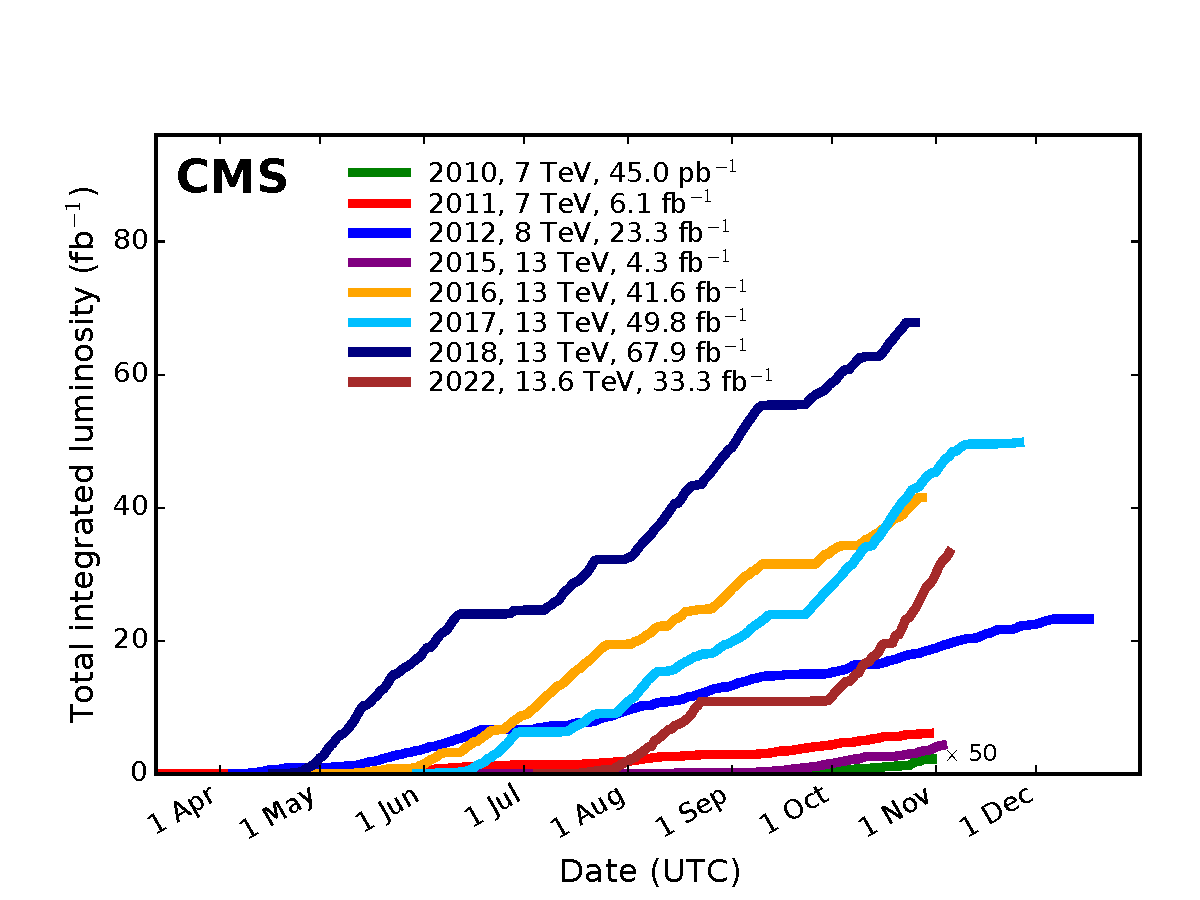
\includegraphics[width=0.34\textwidth]{figs/03_experiment/int_lumi_cumulative_pp_2.pdf}
	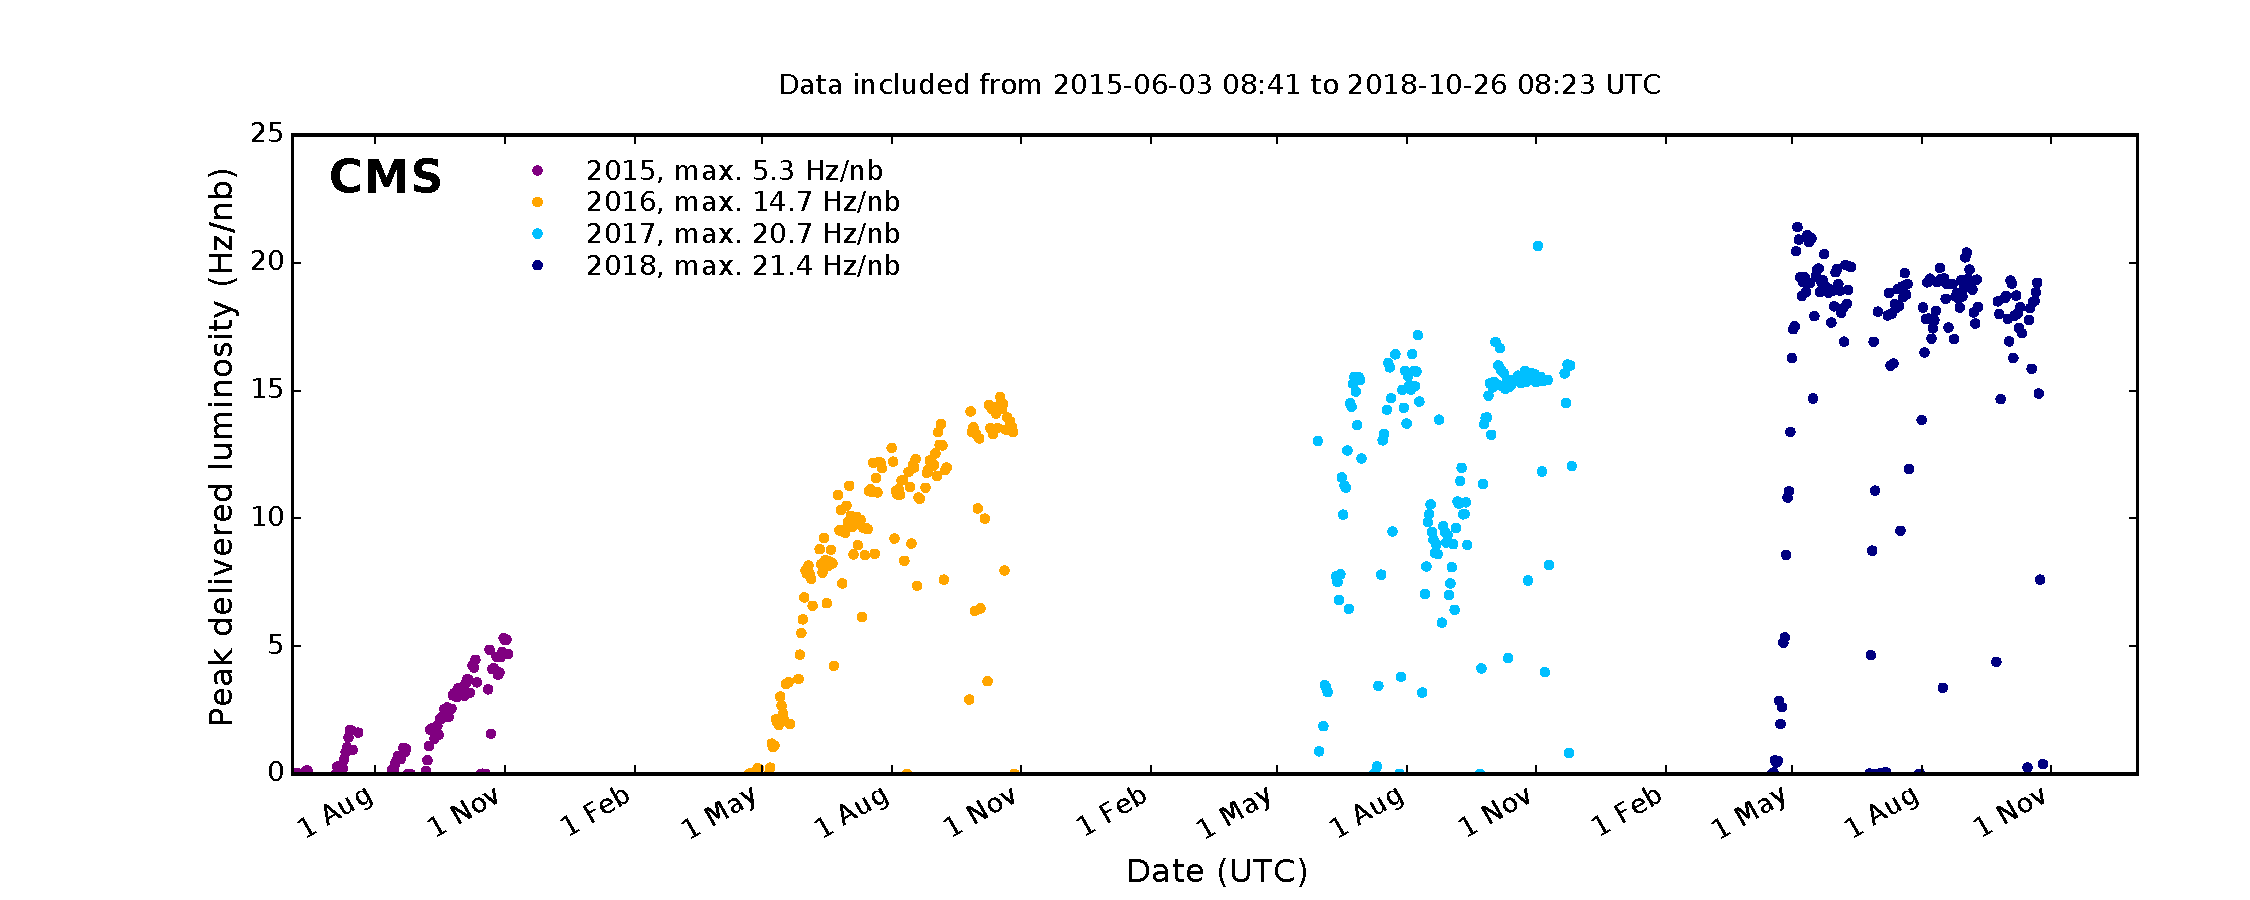
\includegraphics[width=0.65\textwidth]{figs/03_experiment/peak_lumi_pp_run2.pdf}
	\caption[LHC luminosity report. Left: breakdown of the CMS integrated luminosity by year from 2010-2022. Right:  peak luminosity from 2016-2018 data taking~\cite{CMSlumi}.]
	{LHC luminosity report. Left: breakdown of the CMS integrated luminosity by year from 2010-2022. Right: peak instantaneous luminosity from 2016-2018 data taking~\cite{CMSlumi}.}
	\label{fig:LHC_lumi}
\end{figure}

\begin{comment} % Check these numbers? pdg values do not give the correct lumi
\begin{table}[htb!]
	\caption{Description of beam parameters used to calculate the LHC luminosity, obtained from~\cite{Workman:2022ynf} and~\cite{Herr:941318}}
	\begin{center}
		\begin{tabular}{l l l}
			\hline
			Parameter & Description & Value \\
			\hline
			$N_b$ & Number of particles per bunch & $1.1\times10^{11}$\\
			$n_b$ & Number of bunches per event & $2556$\\
			$f_\mathrm{rev}$ & Revolution frequency & $11.245\unit{kHz}$\\
			$\gamma_r$ & Lorentz factor & $6929.6$\\
			$\epsilon_n$ & Transverse normalized beam emittance & $3.75\unit{\mu m\times rad}$\\
			$\beta^*$ & Amplitude function at collision point & $0.3\unit{m}$\\
			$F$ & Geometric luminosity reduction factor & 0.835\\
			\hline
		\end{tabular}
	\end{center}
\end{table}
\end{comment}

% Proton beams
The protons used in collisions are extracted from hydrogen atoms by using ionizing electric fields to strip them of their electrons. Protons are first accelerated to an energy of $50\unit{MeV}$ through a linear accelerator Linac2 before entering the Proton Synchrotron Booster (PSB), where they reach a kinetic energy of $1.4\unit{GeV}$. Next, the protons are accelerated by the Proton Synchrotron (PS) and Super Proton Synchrotron (SPS), where they are accelerated to $26\unit{GeV}$ and $450\unit{GeV}$ respectively. Finally, the beams are injected into the LHC where they undergo acceleration to $6.5\unit{TeV}$, producing the desired center of mass energy of $\sqrt{s}=13\unit{TeV}$.

\begin{figure}[htbp]
	\centering
	\includegraphics[width=0.825\textwidth]{figs/03_experiment/CCC-v2018-print-v2.pdf}
	\caption[Diagram of the CERN accelerator complex during 2018 data taking. Protons begin as hydrogen atoms at Linac2 and collide at various detectors along the LHC at $\sqrt{s}=13\unit{TeV}$]
	{Diagram of the CERN accelerator complex during 2018 data taking~\cite{Mobs:2636343}. Protons begin as hydrogen atoms at Linac2 and are accelerated in several stages to reach $6.5\unit{TeV}$.} 
	\label{fig:LHC}
\end{figure}

\subsection{The High Luminosity LHC} \label{sec:cms_hllhc}
The LHC is designed to go through periods of near continuous data taking, followed by long shut downs during which the detectors undergo various upgrades. As of the time of this writing, the LHC is currently in its third data taking run (Run 3), which is planned to operate from 2022-2025. The end of Run 3 marks the end of Phase-1 and the start of the third long shutdown (LS3), during which the LHC will receive major upgrades to increase the peak instantaneous luminosity up to 75\unit{\hertz\per nb}~\cite{CERN-LHCC-2020-004}, over six times the designed peak luminosity and three times the peak luminosity achieved as of Run 2. The upgraded high luminosity LHC (HL-LHC) will gather substantially more data, which better allows experiments to probe rare processes and measure precise values predicted from the standard model.

\begin{figure} [htbp]
	\centering
	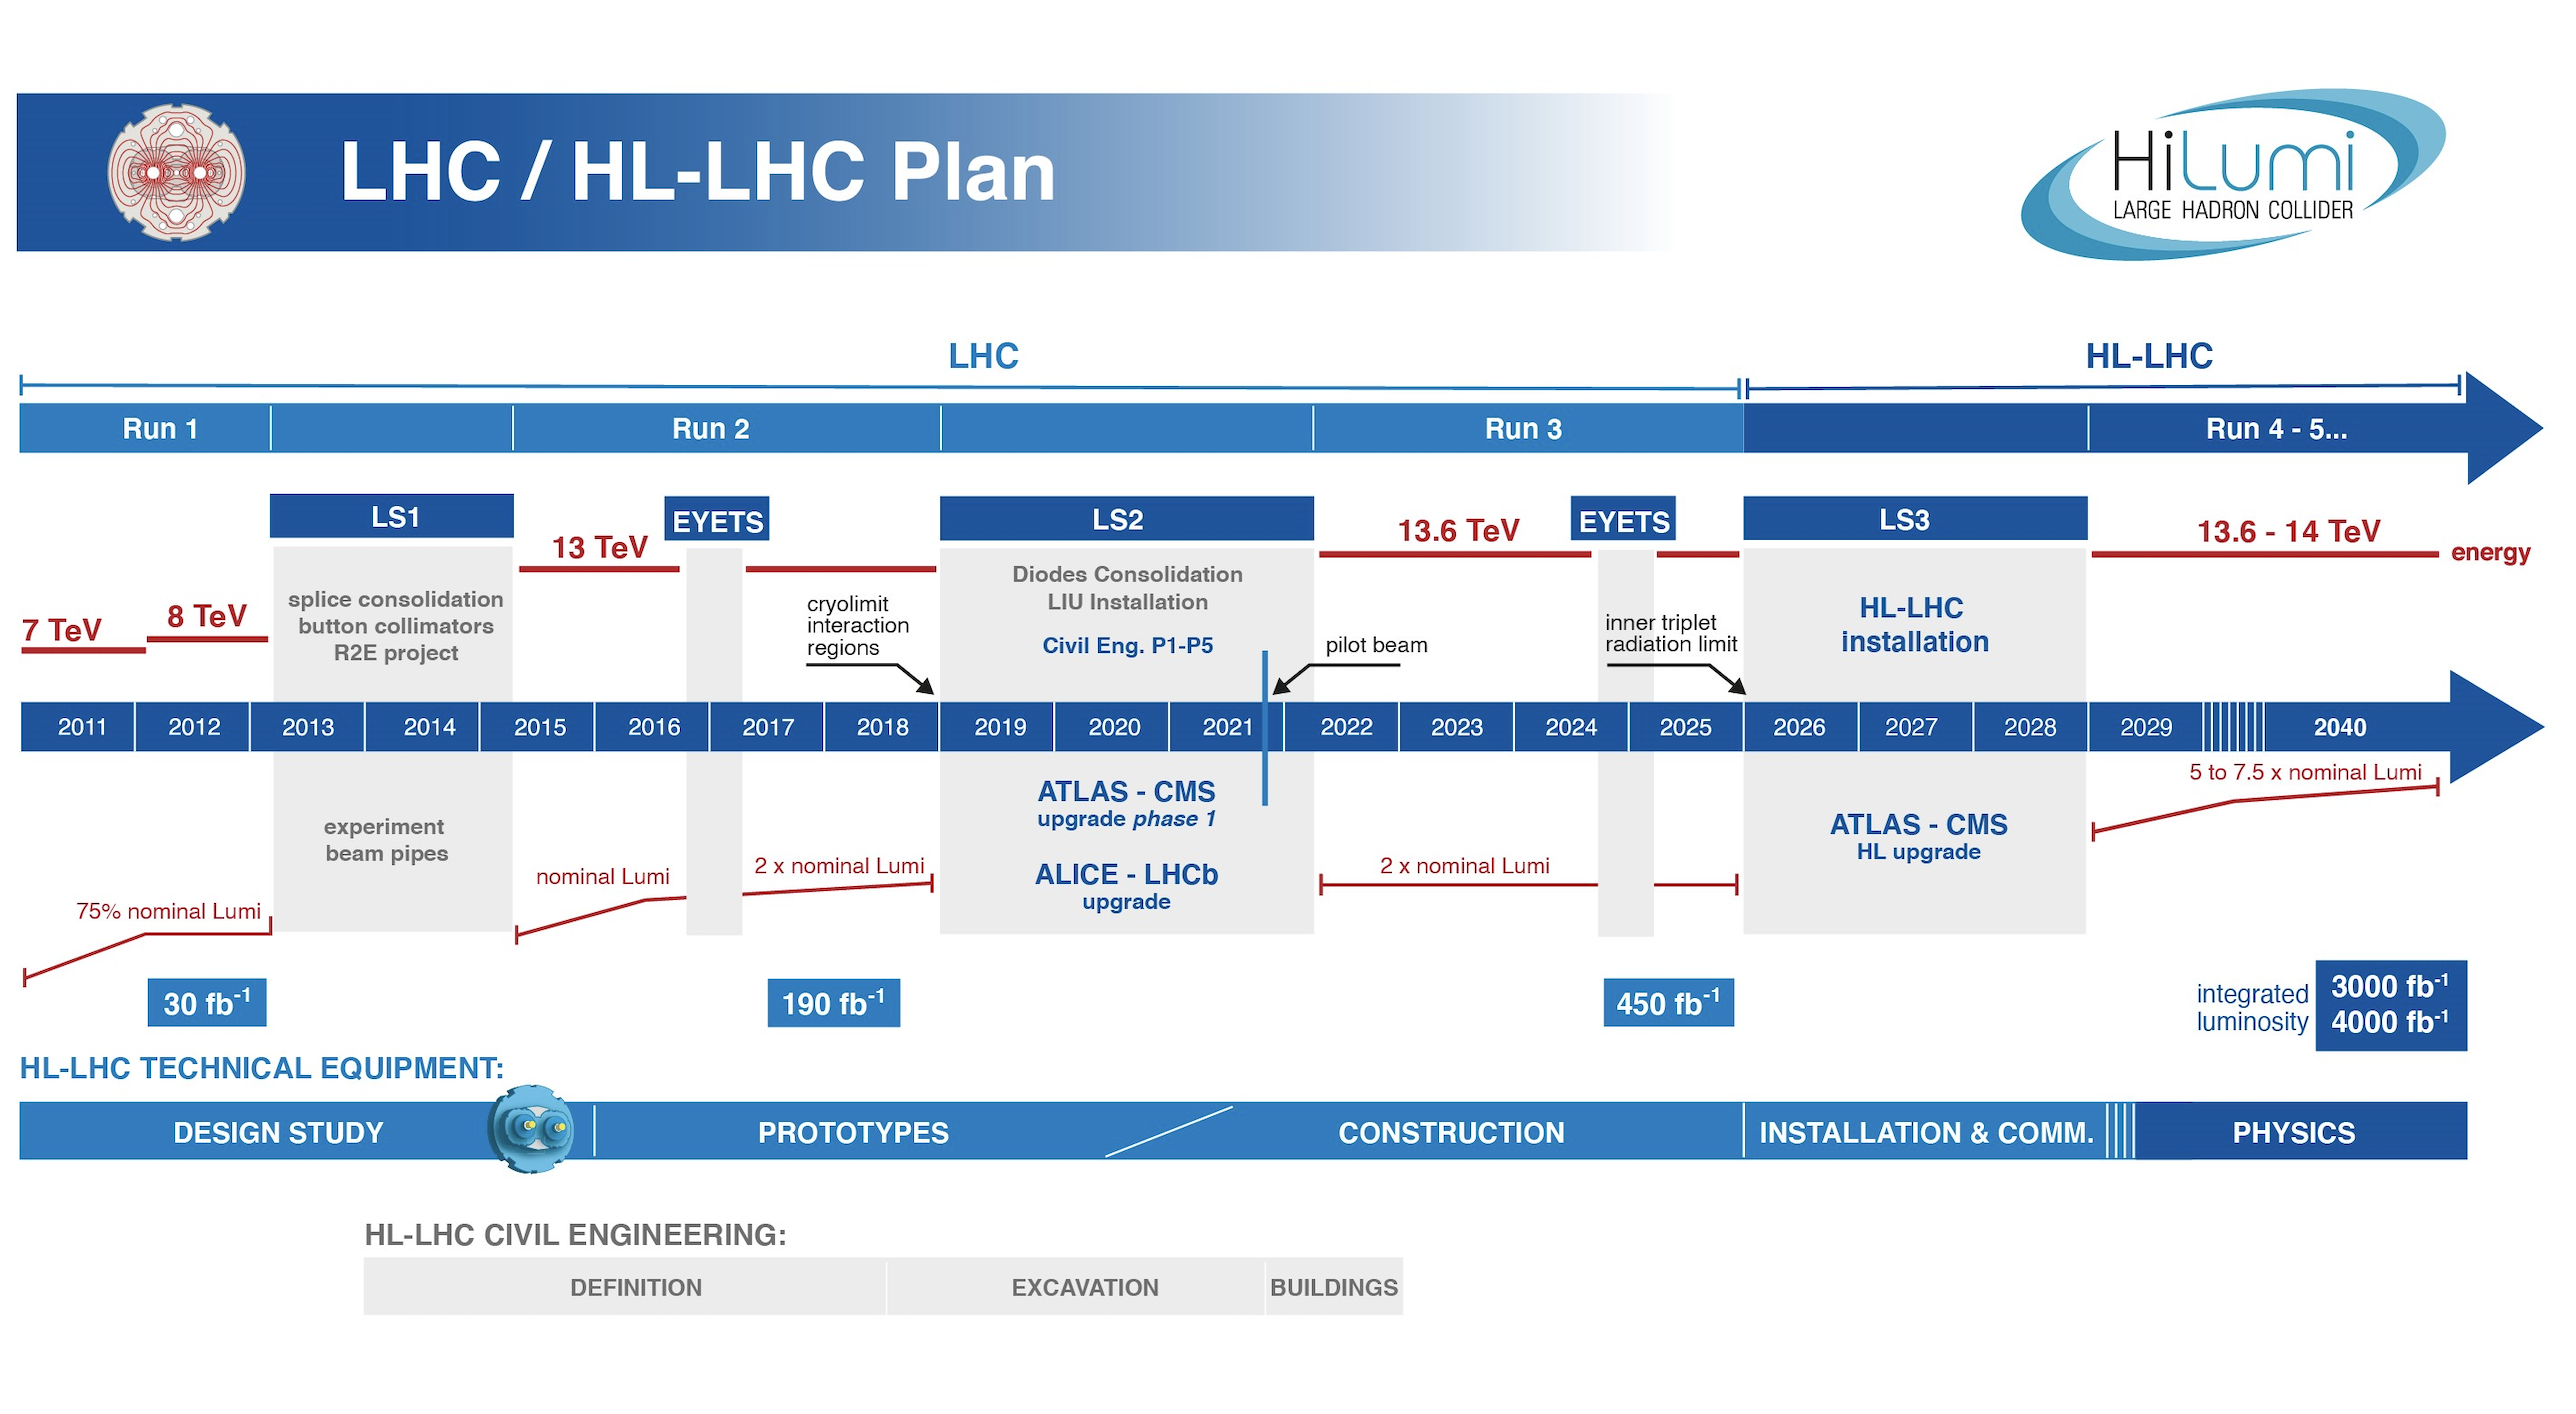
\includegraphics[width=0.84\linewidth]{figs/03_experiment/HLLHCTIMELINE_0.png}
	\caption[Timeline of runs and shutdowns leading to the HL-LHC, showing the improvements to $\sqrt{s}$ and $\lumi$~\cite{HLLHC_timeline}. The extended year-end technical stops (EYETS) are shorter shutdowns generally for routine maintenance, although upgrades such as the CMS Pixel Detector upgrade can occur during this time as well.]{Timeline of runs and shutdowns leading to the HL-LHC, showing the improvements to $\sqrt{s}$ and $\lumi$~\cite{HLLHC_timeline}. The extended year-end technical stops (EYETS) are shorter shutdowns generally for routine maintenance, although upgrades such as the CMS Pixel Detector upgrade can occur during this time as well.}
	\label{fig:HLLHC}
\end{figure}

\section{The Compact Muon Solenoid} \label{sec:CMS}
The Compact Muon Solenoid (CMS) is one of the two general purpose detectors at the LHC, designed to reconstruct physics events from proton-proton collisions. It is a cylindrical apparatus with its major axis aligned with the proton beams from the LHC, consisting of several concentric layers of specialized detectors. The innermost layer consists of a silicon tracker, followed by an electronmagnetic and hadronic calorimeter (ECAL and HCAL, respectively). Surrounding those is the superconducting solenoid, which provides a $3.8\unit{T}$ magnetic field to  the trajectory of charged particles. Lastly, layers of muon chambers are interspaced with an iron return yolk, designed to contain the magnetic field lines near the muon chambers.

\begin{figure}[htbp]
	\centering
	\includegraphics[width=0.9\textwidth]{figs/03_experiment/cms_160312_02.pdf}
	\caption[Cutaway diagram of CMS showcasing major detector components~\cite{Sakuma:2665537}.]
			{Cutaway diagram of CMS showcasing major detector components~\cite{Sakuma:2665537}.}
	\label{fig:CMS}
\end{figure}

\subsection{CMS Coordinate System} \label{sec:CMS_coord}
The origin of the CMS coordinate system is located at the center of the detector, at the nominal collision point of the proton beams. The $+\hat{x}$ axis points radially towards the center of the LHC, while the $+\hat{y}$ axis points vertically upward. This sets the $+\hat{z}$ direction along the beamline, counterclockwise along the LHC. Due to the cylindrical symmetry of CMS, coordinates in the transverse $\hat{x}$-$\hat{y}$ plane are commonly replaced with the radius $r$ and the azimuthal angle $\phi$, which is measured from the positive $\hat{x}$-axis. The polar angle $\theta$ is measured from the $+\hat{z}$-axis, though in practice this variable is rarely used. It is more common to define the polar angle in terms of the pseudorapidity $\eta$, which is defined as
\begin{equation}
	\eta=\frac{1}{2}\ln\left(\frac{|\mathbf{p}|+p_{z}}{|\mathbf{p}|-p_{z}}\right)=-\ln{\tan\left(\frac{\theta}{2}\right)}
\end{equation}
 
The motivation for using $\eta$ instead of $\theta$ stems from a fundamental property of hadron colliders: the center of mass frame for particle production rarely coincides with the lab frame. Thus, when measuring the separation between particles, it is useful to define quantities that remain invariant under Lorentz transformations in the $\hat{z}$ direction. The rapidity $y$ (not to be confused with the Cartesian coordinate $\hat{y}$) is defined as
\begin{equation}
	y=\frac{1}{2}\ln\left(\frac{E+p_{z}}{E-p_{z}}\right)
\end{equation}
It is trivial to show that differences in $y$ remain invariant under Lorentz boosts along the $\hat{z}$-axis. In the highly relativistic limit, which is valid for most particles produced at the LHC, rapidity approaches pseudorapidity as $E\approx|\mathbf{p}|$. The angular separation between two particles can then be expressed as an invariant quantity under Lorentz boots as $\Delta R=\sqrt{\left(\Delta\phi\right)^2+\left(\Delta\eta\right)^2}$. One advantage of pseudorapidity is that $\eta$ can be calculated using only geometric quantities of the detector, whereas $y$ requires calculating both the energy and momenta of a particle, making pseudorapidity the natural choice for defining the polar angle. $\eta$ can range from $\left(-\infty, \infty\right)$, where $\eta=\pm\infty$ points directly along the $\pm\hat{z}$ axis. Higher values of $\left|\eta\right|$ are commonly referred to as "forward".

\subsection{Charged Track Momentum Resolution} \label{sec:CMS_sagitta}
The 3.8\unit{\tesla} magnet curves the trajectory of charged particles, which allows us to precisely determine their momentum. Using the geometry described in section~\ref{sec:CMS_coord}, a particle with charge $q$ and transverse momentum $p_T$ travels in a circular trajectory with radius $R$ when viewed in the $r$-$\phi$ plane. Per the Lorentz Force Law, these can be related by $p_{T} = qBR$. In particle physics, when working with an object of elementary charge, this is commonly rewritten as
\begin{equation}
	\label{eq:pt03br}
	p_{T} = 0.3BR\unit{[GeV/c]}
\end{equation}
The track followed by a charged particle traveling over a length $L$ can be described by the sagitta $s$ shown in figure~\ref{fig:sagitta}, defined by
\begin{equation} \label{eq:sagitta}
	s=R-\sqrt{R^2-\frac{L^2}{4}}
\end{equation}

\begin{figure}[htb!]
	\centering
	% !TEX = root../../thesis.tex
\begin{tikzpicture}
	\def \R{6};
	\def \alpha{30};
	\coordinate (origin) at (0, 0);
	\coordinate (x1) at ({\R*sin(-\alpha)}, {\R*cos(\alpha)});
	\coordinate (x2) at ({\R*sin(\alpha)}, {\R*cos(\alpha)});
	\coordinate (s1) at (0, {\R*cos(\alpha)});
	\coordinate (s2) at (0, \R);
	\draw[dashed] (origin) -- node[below,left]{R} (x1);
	\draw[dashed] (origin) -- (x2);
	\draw (x1) -- node[below]{L/2}(s1);
	\draw (s1) -- (x2);
	\draw (origin) -- (s1);
	\draw (s1) -- node[left]{S} (s2);
	\draw[<-,domain={90-\alpha}:{90+\alpha}] plot ({\R*cos(\x)}, {\R*sin(\x)});
\end{tikzpicture}
	\caption{Diagram showing the sagitta for a charged particle track}
	\label{fig:sagitta}
\end{figure}

For highly energetic particles, the length $L$ is substantially smaller than the radius $R$, so the sagitta can be approximated as
\begin{equation} \label{eq:sagitta_approx}
	s\approx\frac{L^2}{8R}=\frac{0.3BL^2}{8p_T}
\end{equation}

The relative uncertainty of the momentum is proportional to the uncertainty of the sagitta, the track length L, and the magnetic field B as
\begin{equation} \label{eq:dptOverpt}
	\frac{\delta p_T}{p_T}\propto\frac{p_T}{BL^2}\delta s
\end{equation}
The uncertainty on the sagitta $\delta s$ is analogous to the hit resolution of a given detector. Therefore, a long lever arm and high magnetic field strength are crucial to precisely determine the momentum of energetic particles.

\subsection{Inner Tracker} \label{sec:CMS_tracker}
The CMS inner tracker is the first detector surrounding the primary interaction point (IP). Its purpose is to measure the tracks from charged particles as they curve in the strong magnetic field within CMS in order to calculate their momentum and reconstruct secondary vertices. As the closest detector to the primary IP, the tracker experiences the highest particle flux within CMS, and must have high enough granularity to distinguish the multitude of tracks. This high granularity also lends the inner tracker the best momentum resolution for charged tracks out of all the subdetectors comprising CMS, with a momentum resolution of 2.8\% for a 100\unit{GeV} muon~\cite{The_CMS_Collaboration_2014}. The high flux also makes the detector susceptible to radiation damage, so the tracker must be robust in order to maintain efficiency over the long operational period of the LHC. 

The inner tracker utilizes silicon tracking modules composed of P-N type junctions to detect the location of charged particles. When an external voltage is applied to a module, particles passing through will deposit energy and create electron-hole pairs, which drift to their respective electrodes and generate an electrical signal. The applied voltage is tuned such that only a small amount of energy is required to produce electron-hole pairs, which reduces the total amount of material required in order to minimize the energy loss of the charged particles. The inner layer of the tracker is composed of higher granularity pixel detectors, while the outer layer is composed of coarser silicon strips.

\subsubsection{Silicon Pixel Detector} \label{sec:CMS_pixel}
The pixel detector is comprised of 124 million silicon pixel sensors, each with an area of $100\times150\unit{\mu m^2}$ and a thickness of $300\unit{\mu m}$. The barrel (BPIX) consists of four cylindrical layers of pixel sensors spanning from $z=-54\unit{cm}$ to $z=54\unit{cm}$ at radii of $r=2.9$, $6.8$, $10.9$, and $16\unit{cm}$. The endcap (FPIX) consists of three layers located at $z=\pm29.1$, $\pm39.6$, and $\pm51.6\unit{cm}$, which when combined with the barrel nets a total sensitive area of $1.85\unit{m^2}$ with coverage up to $\abs{\eta}<2.5$. With regards to detector performance, the pixel detector provides spatial resolution of $9.5 \unit{\mu m}$ in the $r$-$\phi$ direction and $22.2 \unit{\mu m}$ in the $z$ direction, as well as a hit efficiency of $>99\%$ in each layer at nominal LHC luminosity, with the innermost BPIX layer dropping to $97.5\%$ at peak run 2 efficiency~\cite{CMSPixelP1}.

\begin{figure}[htbp]
	\centering
	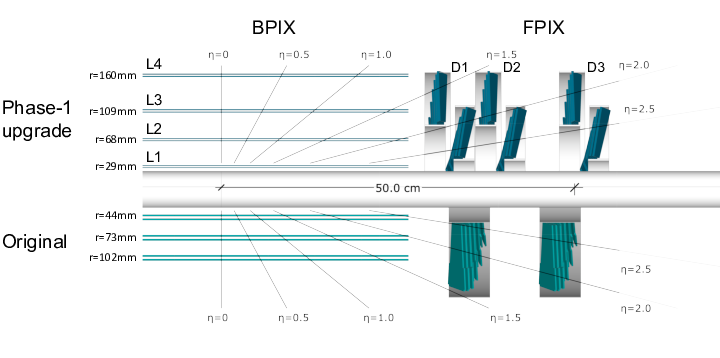
\includegraphics[width=0.85\textwidth]{figs/03_experiment/20120828_01_pixel_phase1_largesharp.png}
	\caption
	[$r$-$z$ slice of the CMS pixel detector~\cite{CMSPixelP1}]
	{$r$-$z$ slice of the CMS pixel detector comparing original design (bottom, teal) with the Phase-I upgrade implemented in 2016/17, which added one layer to both the FPIX and BPIX (top, blue)~\cite{CMSPixelP1}.}
	\label{fig:pixel}
\end{figure}

\subsubsection{Silicon Strip Detector} \label{sec:CMS_strip}
The silicon strip detector surrounds the pixel detector, and is segmented into a tracker inner barrel (TIB), tracker outer barrel (TOB), tracker inner disks (TID), and tracker endcap (TEC). The TIB consists of four layers covering $\left|z\right|<65\unit{cm}$ and radius $25.5\unit{cm}<r<49.8\unit{cm}$. The endcaps of the TIB are covered by the TID, consisting of three disks covering $90<\left|z\right|<90\unit{cm}$. Surrounding the TIB is the TOB, with six layers spanning $\left|z\right|<188\unit{cm}$ and $60.8<\left|r\right|<108\unit{cm}$. Lastly, both the TOB and TID are closed by the TEC, which covers radii ranging from $22<r<113.5\unit{cm}$ and stretches from $124<\left|z\right|<280\unit{cm}$.

The strip detector modules function similarly to the pixel modules, but utilize much larger silicon strips due to the expected reduced particle flux compared to the pixel detector. Each strip detector is composed of $300\unit{\mu m}$ thick micro-strip sensors with pitch varying from $80-205\unit{\mu m}$ to form $7-12.5\unit{cm}$ long strip modules. Overall, the strip detector uses 15,148 modules covering an area of $200\unit{m^2}$ up to $\left|\eta\right|<2.5$.

\begin{figure}[htbp]
	\centering
	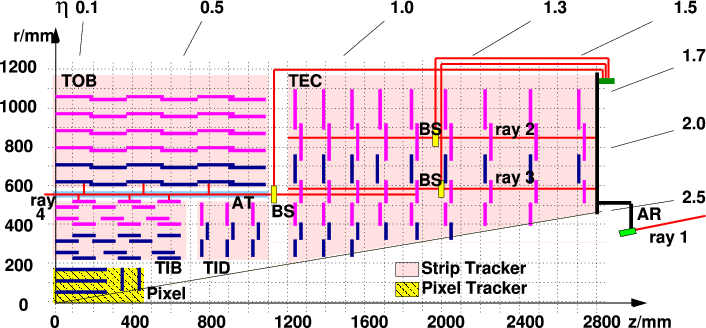
\includegraphics[width=0.85\textwidth]{figs/03_experiment/las.png}
	\caption
	[$r$-$z$ slice of the CMS silicon detector, detailing the four main components of the strip detector~\cite{Chatrchyan:1211825}]
	{$r$-$z$ slice of the CMS silicon detector, detailing the four main components (TIB, TOB, TID, and TEC) of the strip detector. Pixel detector is shown in its Run-I configuration~\cite{Chatrchyan:1211825}.}
	\label{fig:strip}
\end{figure}

\subsection{Electromagnetic Calorimeter} \label{sec:CMS_ECAL}
The CMS Electromagnetic Calorimeter (ECAL) is designed to stop and capture the energy of photons and electrons. When a high energy photon or election enters the ECAL, it primarily interacts with the material in the detector through $e^+e^-$ pair production or bremsstrahlung, respectively. These processes create more photons and electrons that result in an electromagnetic cascade until the particles lose enough energy that ionization and compton scattering processes begin to dominate. This process is known as an electromagnetic shower. The light from these showers is measured using photodetectors to determine the initial energy of the incident particle with resolution given by

\begin{equation}
	\left(\frac{\sigma_E}{E}\right)^2=\left(\frac{2.8\%}{\sqrt{E/\mathrm{GeV}}}\right)^2+\left(\frac{12\%}{E/\mathrm{GeV}}\right)^2+(0.3\%)^2
\end{equation}
The first term arises from statistical fluctuations in the electromagnetic shower and light production, which is a poisson process and therefore proportional to $1/\sqrt{\mathrm{E}}$. The second term is due to the noise in the detector electronics. The last constant term is due to imperfecions in the detector such as non-uniformity, radiation damage, and calibration uncertainty.
The material used for an electromagnetic calorimeter can be characterized by the radiation length ($X_0$) and moli\`ere radius ($R_M$). The radiation length is the average distance an electron will travel before its energy is reduced by a factor of $1/e$, and is roughly proportional to $A/Z^2$, where A is the atomic mass and Z is the atomic number. The moli\`ere radius is directly proportional to the radiation length and measures the spread of an electromagnetic shower in the transverse direction. Both are generally measured in units of $\left[\si{g}\unit{cm^{-2}}\right]$, but can be divided by the density of the material to obtain a distance in $\left[\si{cm}\right]$. A low radiation length and Moli\`ere radius ensure all of the energy is captured in the detector and is contained to a small area to precisely determine the position of an incident particle. It is for this reason that the ECAL is composed of lead-tungstate (PbWO$_4$): a dense, high Z scintillator crystal with $X_0=7.39\unit{g/cm^2}$ (or $0.89\unit{cm}$ after dividing by the density of PbWO$_4$) and $R_M=2.2\unit{cm}$~\cite{Workman:2022ynf}.

The ECAL is constructed from 61200 + 15000 lead-tungstate crystals in the barrel + endcap region. Barrel crystals have a cross sectional area of $2.2\times2.2\unit{cm^2}$ to match the moli\`ere radius and a depth of 23$\unit{cm}$ (or $25.8\,X_0$), and are arranged in rings along the $\phi$ direction, tilted to align with lines of constant $\eta$. The barrel has an inner radius of $129\unit{cm}$ and covers an eta region up to $\left|\eta\right|<1.479$. Endcap crystals have a slightly higher cross sectional area of $2.6\times2.6\unit{cm^2}$ and a slightly lower depth of 22$\unit{cm}$, and are arranged in an $x$-$y$ grid. The endcap provides the remaining coverage from $1.479<\left|\eta\right|<3.0$. A diagram showing the geometry of the ECAL can be seen in figure~\ref{fig:ecal}. The size and alignment of the crystals is designed to contain showers from incident photons/electrons within a $2\times2$ grid of crystals.

One common process in CMS is the production of $\pi^0$s, which decay to two photons. When the two photons deposit their energy into the ECAL, they can fake a signal from a single high energy photon. In order to identify these background events, a higher granularity detector known as a preshower is placed before the ECAL endcap. It consists of a layer of lead absorber to initiate the shower, followed by silicon strip sensors to measure the tracks within the shower. The lead has a thickness of $1.57\unit{cm}$ (or $2.8X_0$), which is thick enough to reliably cause a shower while only causing energy loss of a few percent before the shower can reach the ECAL. The silicon strips are similar to those in the inner tracker, with a pitch of $1.9\unit{mm}$~\cite{TOURNEFIER2001355}.

\begin{figure}[htpb]
	\centering
	\includegraphics[width=0.85\textwidth]{figs/03_experiment/cms_ecal.pdf}
	\caption
	[Geometry of the CMS ECAL showing the barrel, endcap, and preshower, adapted from~\cite{Marzocchi2019}]
	{Geometry of the CMS ECAL showing the barrel, endcap, and preshower, adapted from~\cite{Marzocchi2019}.}
	\label{fig:ecal}
\end{figure}


\subsection{Hadronic Calorimeter} \label{sec:CMS_HCAL}
The CMS Hadronic Calorimeter (HCAL) is a sampling calorimeter surrounding the ECAL. Unlike the ECAL, which is a homogeneous calorimeter where the crystals both induce showers and scintillate, the HCAL is composed of alternating layers of dense absorber and scintillator. The absorber induces hadronic showers - cascades of hadrons resulting from inelastic scattering off a target nuclei. Particles in hadronic showers then pass through the scintillator, which produces light that gets transmitted through wavelength shifting fibers and read out by photodetectors, before repeating this process with the next layer of absorber/scintillator. The measured energy can be summed in sequential layers of detectors (referred to as "towers") to calculate the total energy of the incident hadron. As an additional complication, several hadrons decay to electrons or photons, which will create electromagnetic showers, requiring the scintillator to have good response to electromagnetic interactions. The HCAL must be hermetic, as a complete picture of the energy from proton collisions is required to infer the production of particles like neutrinos, which are otherwise invisible to the detector.

The relevant property for a hadronic absorber is the nuclear interaction length $\lambda_I$, which is the mean distance a hadron will travel before undergoing an inelastic nuclear interaction. Like the radiation length, $\lambda_I$ is measured in $\left[\si{\gram\ \centi\metre^{-2}}\right]$ and can be divided by the density to obtain a distance in $\left[\si{\centi\meter}\right]$. It is proportional to the density of nuclear matter, which goes as $\text{A}^{1/3}$. The HCAL uses a combination of brass and stainless steel, which have an interaction length of $\sim16.5\unit{cm}$~\cite{Baiatian:1049915}.

The HCAL consists of four subsystems: an inner barrel (HB), an outer barrel (HO), an endcap (HE), and a forward calorimeter (HF). The HB covers $\left|\eta\right|<1.3$ with 36 azimuthal wedges, each containing 17 layers of alternating brass absorber and scintillator. These wedges begin at a radius of $1.806\unit{m}$ and are $89\unit{cm}$ thick, resulting in a minimum of $5.3\,\lambda_I$ at $\eta=0$, increasing to $10\,\lambda_I$ and $\eta=1.2$. The HE consists of two disks, also formed of 36 wedges with 19 layers of brass absorber and scintillator, totaling 10 $\lambda_I$ in order to contain highly boosted, forward showers resulting from quarks and gluons.. The HE extends the coverage of the HCAL up to $\left|\eta\right| < 3.0$. The HO is located outside the magnetic coil to catch high energy ($>100\unit{GeV}$) hadrons that escape the HB. It consists of five rings in eta, covering up to $\left|\eta\right|<1.2$, and relies on the iron solenoid to induce hadronic showers. The HF covers the most forward region of $3<\left|\eta\right|<5$. This zone has the highest exposure of radiation, and so the detector must be sensitive only to the highest energy particles and robust against damage from heavy radiation. It uses steel as the absorber and quartz fibers to scintillate through Cherenkov radiation. The four subsystems provides a minimum of $10\,\lambda$ to capture incident hadrons.

\begin{figure}[htpb]
	\centering
	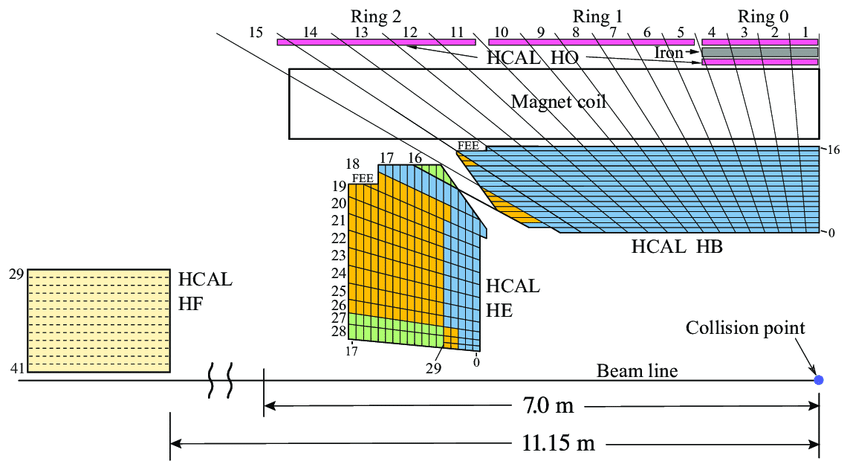
\includegraphics[width=0.85\textwidth]{figs/03_experiment/A-schematic-view-of-one-quarter-of-the-CMS-HCAL-during-2016-LHC-operation-showing-the.png}
	\caption
	[$r$-$z$ slice of the CMS HCAL showing the HB, HE, HF, and HO~\cite{Sirunyan:2691403}]
	{$r$-$z$ slice of the CMS HCAL showing the HB, HE, HF, and HO~\cite{Sirunyan:2691403}.}
	\label{fig:hcal}
\end{figure}

\subsection{Muon Detectors} \label{sec:CMS_Muons}
The muon chambers lie outside the magnetic solenoid as the outermost subsystem in CMS. Due to the distance and amount of material between them and the primary IP, they are the lowest occupancy detectors, with few particles other than muons able to reach them before decaying or stopping in the inner subsystems. Although they lie outside the solenoid, the iron yolk pulls the magnetic field back to curve the trajectory of muons, which is required calculate their momenta. The detector subsystem is composed of three types of gaseous detection chambers: drift tubes (DTs), resistive plate chambers (RPCs), and cathode strip chambers (CSCs). A diagram showing the configuration of these detection chambers can be seen in figure~\ref{fig:Muons}.

The operating physics principles of all three chambers are similar: muons pass through a gas mixture and ionize the gas, knocking loose electrons. Anodes and cathodes create an electric field inside the gas chamber, causing the electrons to drift to the anode where they can be measured and read out by electronics. Electrons that are excited but not ionized from the incident muon will emit photons as they transition back to a lower energy level, thus a quenching gas is used to absorb these photons to prevent further cascades. The specifics of the three detectors are described in sections~\ref{sec:CMS_DT}-\ref{sec:CMS_RPC}.

\begin{figure}[htpb]
	\centering
	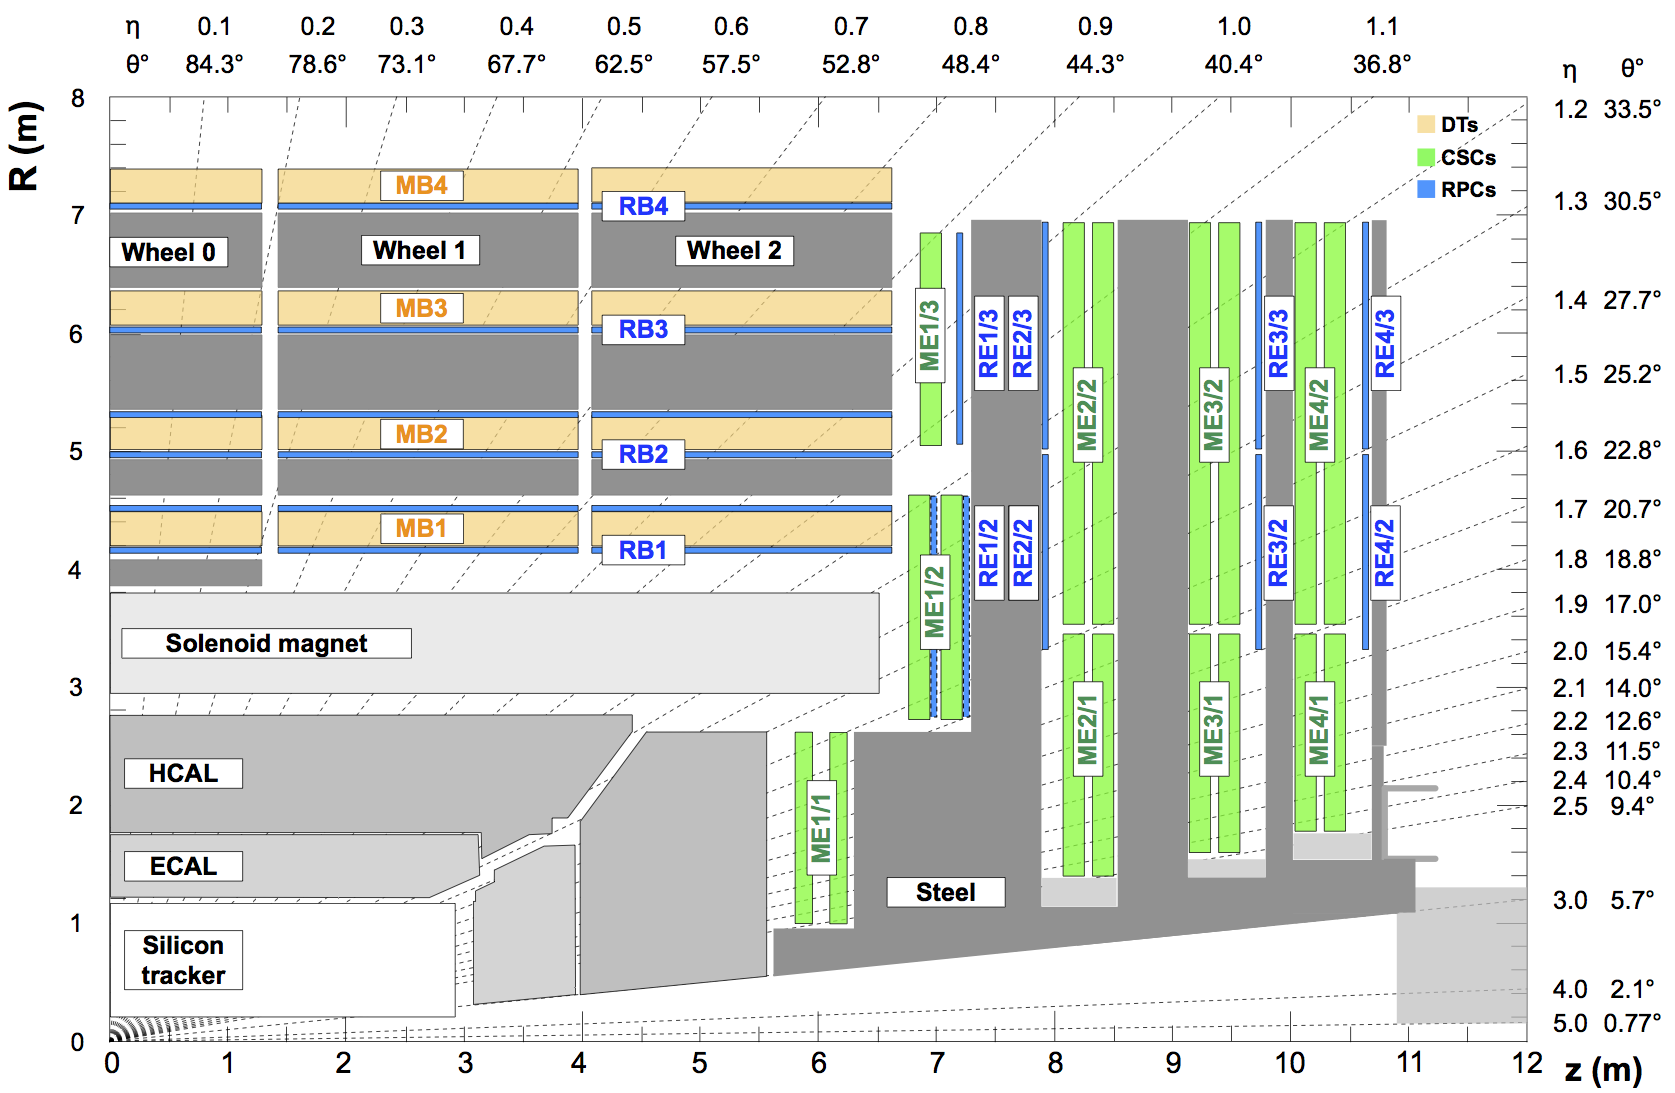
\includegraphics[width=0.85\textwidth]{figs/03_experiment/Muon_system.png}
	\caption
	[Diagram of the CMS Muon system~\cite{Sirunyan:2313130}]
	{$r$-$z$ cross section of the CMS muon detector subsystem, configured for the 2016-2018 data taking run. The barrel consists of five wheels of DTs and RPCs in $\eta$, each wheel consisting of four layers in $r$ and 12 sectors in $\phi$, covering up to $\left|\eta\right| < 1.2$. The endcap consists of four layers of DTs and RPCs in $z$~\cite{Sirunyan:2313130}.}
	\label{fig:Muons}
\end{figure}

\subsubsection{Drift Tubes} \label{sec:CMS_DT}
Drift tubes are used in the barrel of the muon system, covering $\left|\eta\right| < 1.2$. They consist of long chambers filled with an mixture of Ar/$\text{CO}_2$, with an anode wire running lengthwise through the center and cathode strips along the edges. Electrode strips along the outer edge of the chamber shape the electric field lines to linearize the drift velocity of electrons throughout the chamber. When a muon passes through the chamber, ionized electrons follow the electric field lines towards the anode wire. Due to the known field inside the chamber, the drift time can be used to calculate the transverse distance from the wire to the incident muon with a resolution of $250\unit{\mu\m}$. The DTs are arranged in superlayers, which consist of 4 layers of DTs, with subsequent superlayers alternating in the $r$-$z$ and $r$-$\phi$ direction in order to obtain the muon trajectory/curvature in both the $\eta$ and $\phi$ direction. Figure~\ref{fig:DT} shows a diagram of a DT superlayer and a single DT cell.

\begin{figure}[htpb]
	\centering
	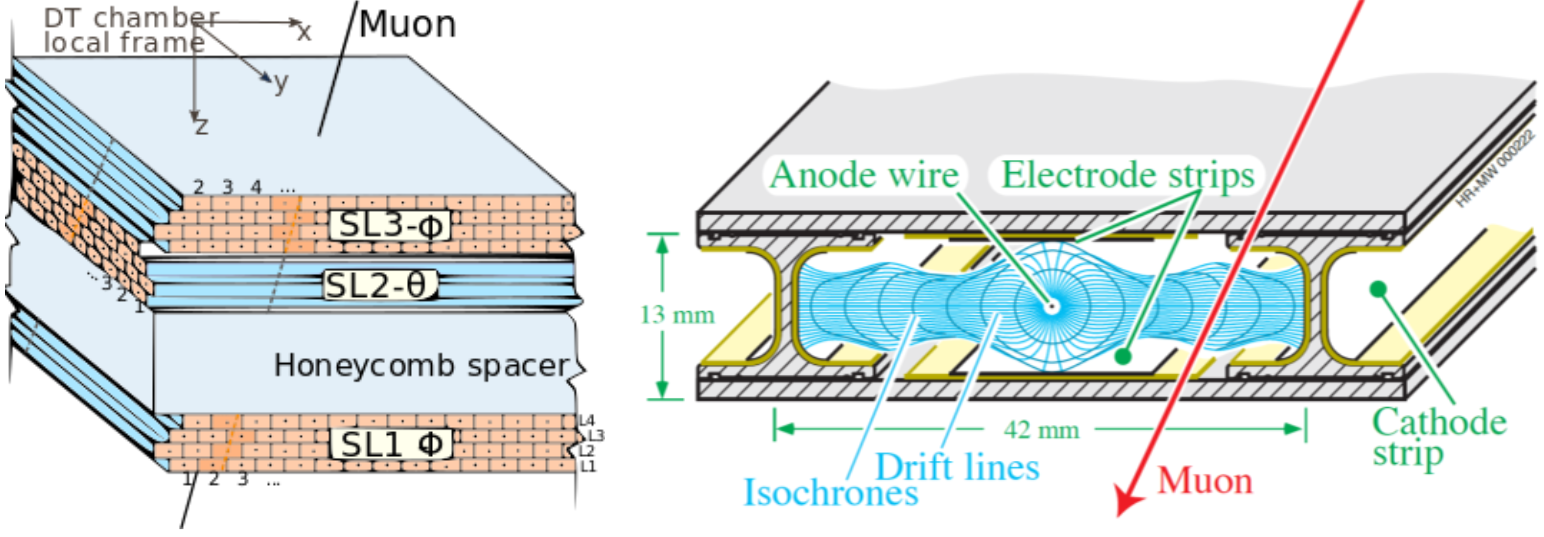
\includegraphics[width=0.85\textwidth]{figs/03_experiment/CMS_DT.png}
	\caption
	[Diagram of the CMS Drift Tubes~\cite{CMSDT}]
	{Drift tube superlayers are aligned in alternating orientations in order to provide a complete picture of muon trajectories (left). A cross section of a single drift tube chamber (right). Electrons ionized from the muon drift to the anode wire to produce a measurable current~\cite{CMSDT}.}
	\label{fig:DT}
\end{figure}

\subsubsection{Cathode Strip Chambers} \label{sec:CMS_CSC}
Cathode strip chambers are used in the endcaps of the muon system to provide coverage from $0.9<\left|\eta\right|<2.4$. CSC modules are trapezoidal chambers filled with a mixture of Ar/$\text{CO}_2$/$\text{CF}_4$ and arranged in disks to cover the muon endcap. Each module is composed of six layers of radial cathode strips, which have high granularity in $\phi$, and transverse anode wires which provide granularity in $r$. Similar to the DTs, muons passing through CSC chambers ionize the gas molecules, knocking loose electrons which drift to the anode wires. The charge from these electrons can is measured and provides the position of the muon in $r$. Simultaneously, the electrons induce a charge in the cathode strips, which provides the position of the muon in $\phi$. One chamber provides a spatial resolution of between $40-50\unit{\mu m}$ with a time resolution of $3\unit{ns}$.

\begin{figure}[htpb]
	\centering
	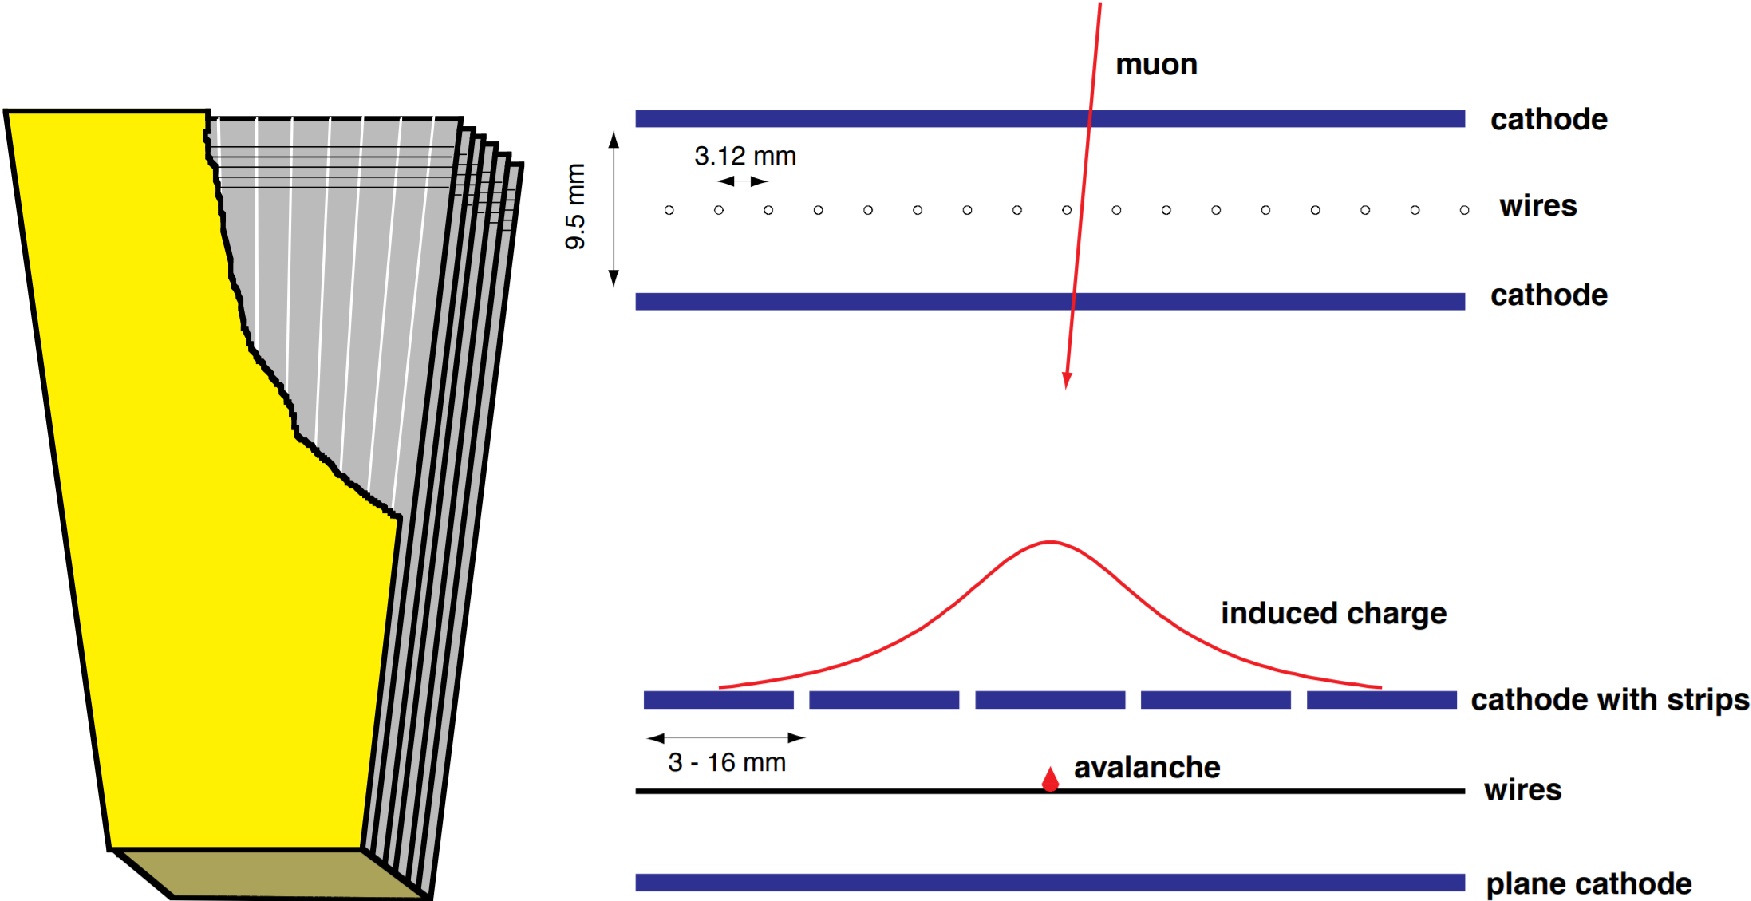
\includegraphics[width=0.85\textwidth]{figs/03_experiment/cms_csc.pdf}
	\caption
	[Cut-away diagram of a single CSC module~\cite{DeBruyn:2797803}]
	{Cut-away diagram of a single CSC module showing the six layers of radial cathode strips and transverse anode wires (left). Muons ionize the gas chamber, causing an avalanche of electrons on the anode wires and inducing a charge on the cathode strips (right)~\cite{DeBruyn:2797803}.}
	\label{fig:CSC}
\end{figure}

\subsubsection{Resistive Plate Chambers} \label{sec:CMS_RPC}
RPC detectors are used in conjunction with the DTs and CSCs in both the barrel and endcap. One RPC consists of two high resistivity plastic plates: one positively charged anode and a negatively charged cathode which create a strong, uniform electric feel between the two. The space between the two plates is filled with a mixture of 95\% C$_2$H$_2$F$_4$ and 5\% iso-C$_4$H$_{10}$. Incident muons ionize the gas between the two plates, which cause a cascade of electrons towards the anode plate due to the strong electric field. External metal strips lie outside the anode in order to measure the avalanche of electrons. The coarse nature of the strips means the RPC spatial resolution is lower than that of the CSCs and DTs at around $1\unit{cm}$, but the time resolution is much faster on the order of $1\unit{ns}$. For this reason they are used to supplement the CSC and DTs to aid with triggering and accurate timing.

\begin{figure}[htpb]
	\centering
	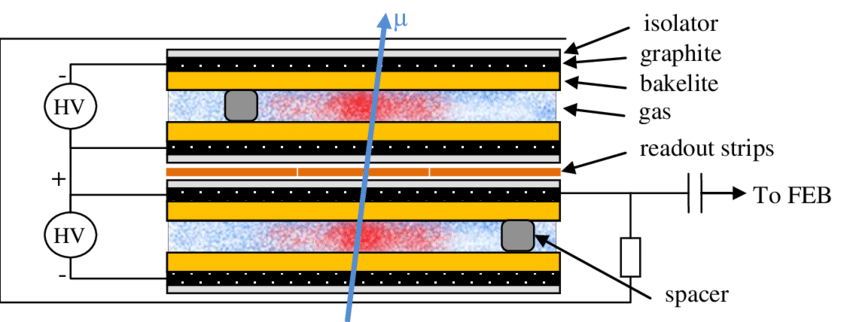
\includegraphics[width=0.85\textwidth]{figs/03_experiment/Design1.png}
	\caption
	[Diagram of the double RPC at CMS~\cite{CMSRPC_HLLHC}]
	{Diagram of the double RPC at CMS. Incident muons ionize the gas, causing a cascade of electrons towards the readout strips~\cite{CMSRPC_HLLHC}.}
	\label{fig:RPC}
\end{figure}

\subsection{Trigger System} \label{sec:CMS_trig}
The high luminosity of the LHC yields an incredibly high rate of information to store from the various detectors. Each event contains approximately $1\unit{MB}$ of data to store, which would take bandwidth and storage space beyond current capacities to save given the $40\unit{MHz}$ collision rate. Additionally, many events are soft collisions that do not contain interesting physics worth storing for further analysis. In order to reduce the rate of events and select only the most interesting collisions, CMS employs a two level trigger system. The first level is known as the Level-1 (L1) trigger and uses hardware to identify physics objects in real time. The second is known as the High-Level trigger (HLT), consisting of a conventional CPU farm which performs more advanced calculations.

\subsubsection{Level-1 Trigger} \label{sec:CMS_L1T}
The L1 trigger utilizes special processors such as Field Programmable Gate Arrays (FPGAs) in order to process coarse information from the calorimeters and muon chambers in real time. The coarse detector information, known as trigger primitives, is subjected to several algorithms to create physics objects (e.g. muons, electrons/photons, etc). Objects passing a predetermined set of criteria are called trigger "seeds", with events that satisfy at least one seed getting passed to the HLT. A diagram of the L1 trigger architecture can be seen in figure~\ref{fig:L1T}. This entire decision making process must take place in $3.2\unit{\mu s}$ after a bunch crossing. As this is greater than the time between bunch crossings, the L1 trigger must be pipelined in order to operate continuously, while the full data is kept in a rolling buffer and read out only if the event passes a trigger seed. The L1 trigger was designed to accept events at a maximum rate of about $100\unit{kHz}$, meaning only one in every four hundred events is passed to the HLT.

\begin{figure}[htpb]
	\centering
	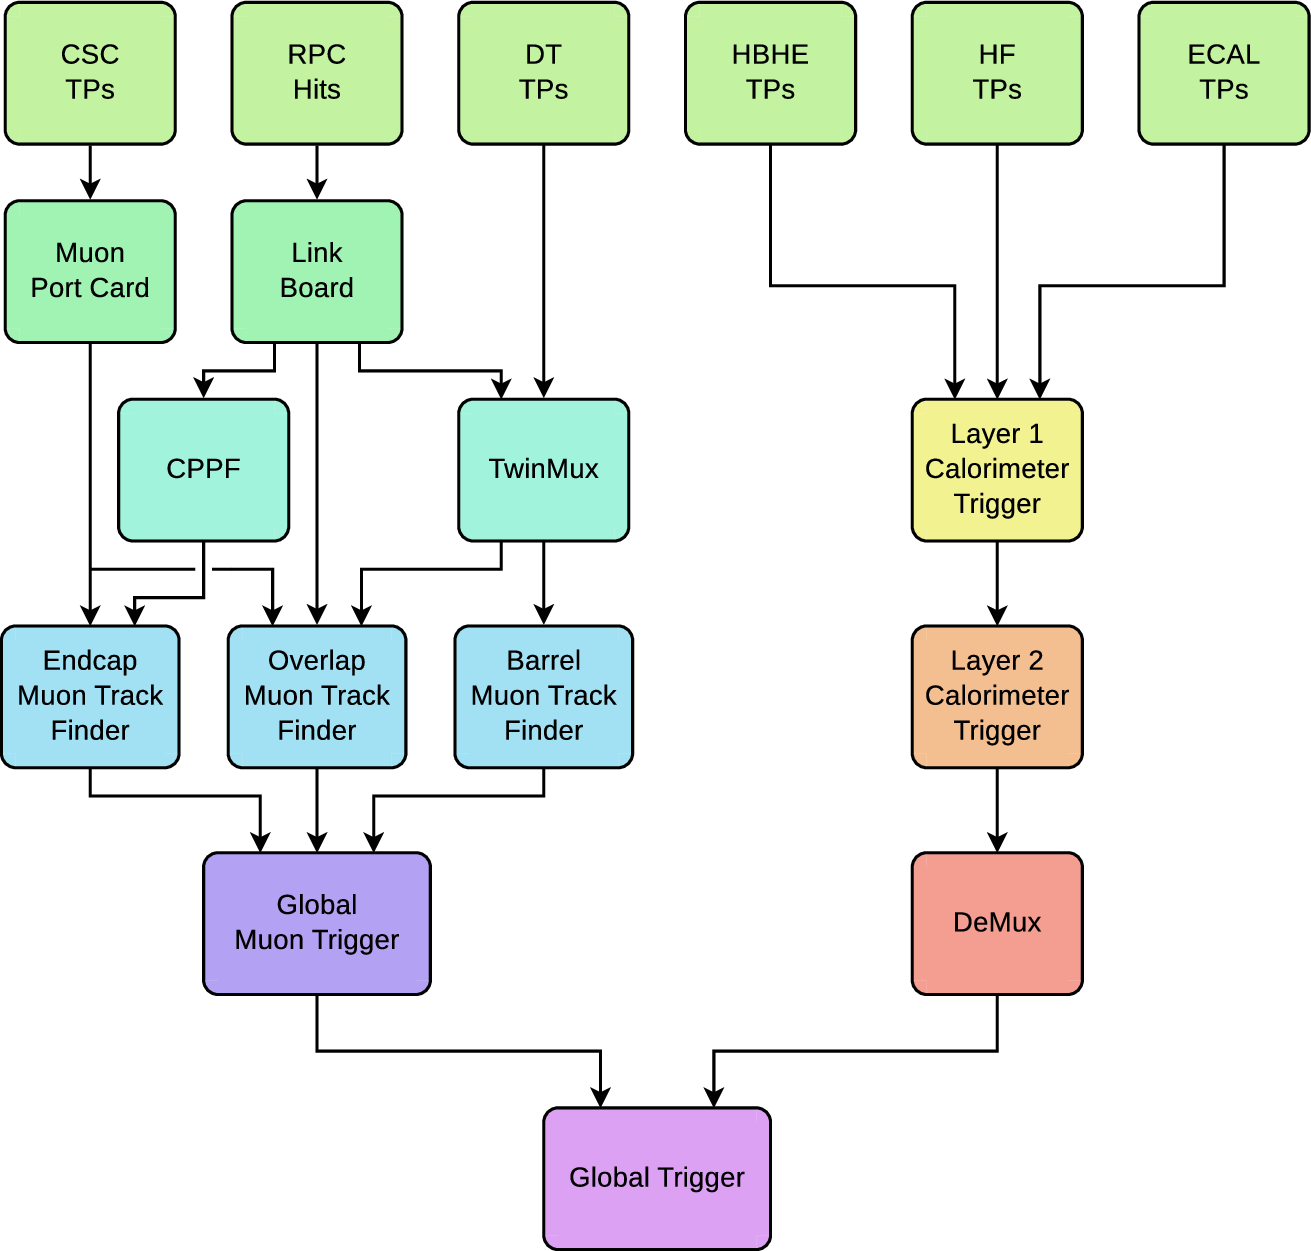
\includegraphics[width=0.55\textwidth]{figs/03_experiment/cms_l1t.png}
	\caption[CMS Level-1 Trigger architecture during Run 2~\cite{Sirunyan:2721198}]
	{Block diagram of the CMS Level-1 Trigger architecture during Run 2~\cite{Sirunyan:2721198}. Muon objects found in the barrel, overlap, and endcap regions are ranked and sorted using their momentum and quality criteria before being passed to the Global Muon Trigger (GMT), which cleans duplicate tracks and selects the top eight muons. The muons are then passed to the global trigger, which combines the muons with objects created from the calorimeters and makes the final decision to pass the event to the HLT.}
	\label{fig:L1T}
\end{figure}

The L1 trigger will undergo several changes during LS3 as a result of the HL-LHC upgrade discussed in section~\ref{sec:cms_hllhc}. The main consequence of higher luminosity is an increase in additional proton collisions along the beamline per bunch crossing, known as pileup. Interesting physics events generally stem from a single hard scattering interaction, known as the primary vertex (PV), with lower energy pileup collisions creating background that can obscure the physics from the PV. The L1 trigger is well equipped for the average 40 pileup for Run 3, but will require upgrades in order to accommodate the expected 200 pileup for the HL-LHC. As part of the L1 trigger update, the maximum bandwidth will be increased from $100\unit{\kilo\hertz}$ to $750\unit{\kilo\hertz}$ and the trigger decision latency will be increased from $3.2\unit{\micro\second}$ to $12.5\unit{\micro\second}$. Additionally, new tracker primitives will be available as inputs to the calorimeters and muon triggers. These primitives allow the precise $p_T$, $\eta$, and $\phi$ information from tracks to be associated with calorimeter clusters and muon primitives, greatly increasing the precision and efficiency of L1 reconstruction. The proposed trigger architecture for the HL-LHC can be seen in figure~\ref{fig:HL_L1_trig}.

\begin{figure} [htbp]
	\centering
	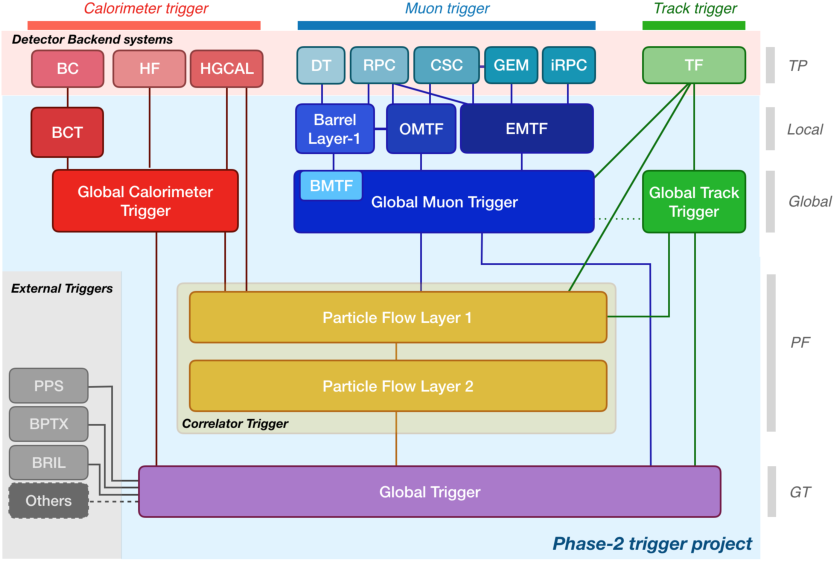
\includegraphics[width=0.65\linewidth]{figs/03_experiment/HLLHC_L1T.png}
	\caption[Designed trigger architecture of the HL-LHC. The addition of the track primitives allows the computation of more advanced reconstruction algorithms at the L1 level~\cite{inproceedings}.]{Designed trigger architecture of the HL-LHC. The addition of the track primitives allows the computation of more advanced reconstruction algorithms at the L1 level~\cite{inproceedings}.} 
	\label{fig:HL_L1_trig}
\end{figure}

\subsubsection{High Level Trigger} \label{sec:CMS_HLT}
The HLT receives the full precision detector data for events passing the L1 trigger, and is designed to reduce the final event rate to approximately $100\unit{Hz}$, five orders of magnitude less than the LHC bunch crossing rate. Information from the tracker allows the HLT algorithms to reconstruct a more complete picture of an event, as tracker information can be matched to both calorimeter hits and muon tracks to provide more detail to reconstructed physics objects. As with the L1 trigger, the HLT processes data through a series of trigger paths, which sequentially reconstruct and filter physics objects. In order to optimize computation time, the HLT uses L1 trigger seed to inform which trigger paths to use, and structures the paths in order of increasing complexity. For example, electrons are first created using only calorimeter data, then matched using coarse hits in the tracker, before being reconstructed using full tracker information. Events passing the HLT are then recorded permanently for offline reconstruction and analysis. 

\subsection{Event Reconstruction} \label{sec:CMS_Reco}
Events that pass the HLT then undergo a complete event reconstruction, where data from all sub-detectors is combined to identify each physics object created in a collision. This section provides an description of the relevant objects for this dissertation, namely muons, electrons, and photons, as well as a brief description of the particle flow (PF) algorithm used for global event reconstruction.

\subsubsection{Tracks and Calorimeter Clusters} \label{sec:CMS_trk_clusters}
Raw detector information taken from the inner tracker and calorimeter are used to create tracks and clusters, which are the building blocks used to create a global event reconstruction. Tracks are built using a Kalman Filter algorithm to fit particle trajectories to hits in the pixel and strip detectors. This process begins with a track seed which is built from hits in the pixel detector compatible with a charged particle track. The initial seed track is propagated outward to collect nearby hits in successive layers of the tracker. Once the seed and hits are collected, the track is iteratively fit to determine the final properties of the charged particle, namely the origin, $\pt$, and direction. Various quality cuts are applied based on the number of hits in order to reject fake or misidentified tracks.

Clusters are seeded from individual cells in the calorimeters with an energy above a preset threshold. Adjacent cells are added to the cluster if they have an energy above twice the expected noise level to form superclusters. The average noise level per cell in the electromagnetic calorimeter is roughly 40 and 150 MeV in the barrel and endcap respectively, while the noise per tower in the hadronic calorimeter is around 200 MeV~\cite{Sirunyan:PF}. Lastly, various algorithms calculate the substructure of these topological clusters to separate contributions from individual sources into smaller clusters.

\subsubsection{Muon Reconstruction} \label{sec:CMS_Reco_mu}
Muon reconstruction relies on tracks reconstructed in the inner tracker (tracker tracks) and tracks reconstructed in the muon systems. There are three categories of muon objects based on the method used to reconstruct tracks.

\textit{Standalone-muon tracks} utilize a Kalman-filter algorithm to construct tracks using only information from the muon system. Tracks seeds are formed from CSC or DT track segments and propagated to nearby hits in the muon chambers.

\textit{Global muon tracks} begin with a standalone track, which is propagated to the silicon tracker and matched to compatible tracker tracks. Two tracks are matched if the standalone track and tracker track can be propagated to a common surface. The track is then refit using a Kalman filter by combining the information from the tracker and standalone track. 

\textit{Tracker muon tracks} recapture muons in detector gaps and lower p$_T$ muons that leave hits in the muon chambers but do not fully penetrate the muon system. In these cases, it is common for a muon to leave a segment of hits in consecutive DT/CSC layers that are compatible with a track but not produce a standalone track. Tracker muons are formed by propagating all tracker tracks with p$_T > 0.5\unit{GeV}$ and p $>2.5\unit{GeV}$ into the muon chambers, and matching to nearby muon segments.

This reconstruction has an efficiency of 99\% for muons produced within the geometric acceptance of the muon system\cite{Sirunyan:2313130}. Muon objects are then fed into the PF algorithm, which performs selection criteria based on the quality of the track. As the purity of each track varies based on type (e.g. hadrons that "punch through" the HCAL are more probable to be reconstructed as track muon tracks), the cuts vary for each category.

\subsubsection{Electron and Photon Reconstruction} \label{sec:CMS_reco_egamma}
In theory, electrons should leave a smoothly curving track in the silicon tracker and deposit nearly all of their energy within a few crystals in the ECAL. However in practice, electrons frequently interact with the material in the tracker, which induces electromagnetic showers before the particle can reach the calorimeter, resulting in tracks which can have sudden changes in curvature and ECAL clusters that are smeared in $\phi$.

The e/$\gamma$ reconstruction algorithm accounts for these factors when track fitting and forming clusters for electrons. Electron track seeds are formed when the momentum of a track and the energy of an associated ECAL cluster are compatible with unity~\cite{Sirunyan:PF}. These tracks are refit using a Gaussian Sum Filter (GSF), which uses a sum of gaussian distributions to approximate the probability density function for energy loss due to bremsstrahlung~\cite{Adam_2005}.

Bremsstrahlung photons are emitted tangent to the trajectory of the electron, which bends in $\phi$. To ensure this energy is accounted for in the reconstruction, clusters located tangent to the GSF track are associated to the track and supercluster. Additionally, the total cluster energy is calibrated as a function of energy and $\eta$ to account for energy loss. Photons, which are seeded by ECAL clusters with no linked GSF track, can undergo the same process of pair production to induce electromagnetic showers. As such, photon candidate clusters are subject to the same energy calibration.

Several cuts are applied to the candidate particles to reject background from hadronic processes. Electrons and photons are expected to have a low ratio of linked HCAL cluster energy to their ECAL cluster energy. Electron tracks have several variables that are fed to a boosted decision tree, which decides whether or not to accept an electron candidate. All tracks, GSR tracks, clusters, and superclusters associated with reconstructed electrons or photons are passed to the PF algorithm.

\subsubsection{Particle Flow} \label{sec:CMS_PF}
Particle flow (PF) is a global reconstruction algorithm that takes advantage of the unique signatures of various physics objects as they pass through each detector. It takes information passed from the muon, electron, and photon reconstruction as well as the remaining tracks and clusters as input to form "pf blocks" in a process known as linking, which topologically associates objects from one or more detector. The particle flow algorithm then takes these blocks and reconstructs the individual particles. In order, the algorithm reconstructs muons, electrons and isolated photons, charged hadrons, and neutral particles. After each step the corresponding tracks and clusters are removed from the pf blocks to prevent double counting. Once all objects are reconstructed, a final post processing step is done to further reduce mis-reconstructed particles. The PF candidates are used to reconstruct higher level objects such as hadronized quarks and gluons, decay products from $\tau$ mesons, or $b$-quark decays, and calculate the imbalance of transverse momentum created from particles that are invisible to the detector (called missing E$_T$, or MET).